% !TeX TXS-program:compile = txs:///pdflatex/[--shell-escape]
\documentclass[10pt,landscape,a4paper]{article}
\usepackage[table]{xcolor}
\usepackage[normalem]{ulem}
\usepackage{tikz}
\usetikzlibrary{shapes,positioning,arrows,fit,calc,graphs,graphs.standard}
\usepackage[nosf]{kpfonts}
\usepackage[t1]{sourcesanspro}
\usepackage{multicol}
\usepackage{wrapfig}
\usepackage[top=1mm,bottom=1mm,left=1mm,right=1mm]{geometry}
\usepackage[framemethod=tikz]{mdframed}
\usepackage{microtype}
\usepackage{tabularx}
\usepackage{hhline}
\usepackage{makecell}
\usepackage{mathtools}
\usepackage{subfig}
\usepackage{listings}
\usepackage{soul}
\usepackage{amsmath,amsthm,amsfonts,amssymb}

\graphicspath{ {./img/} }

\DeclarePairedDelimiter{\ceil}{\lceil}{\rceil}

\newcommand\codeblue[1]{\textcolor{blue}{\code{#1}}}

\definecolor{myblue}{cmyk}{1,.72,0,.38}
\definecolor{LightGray}{gray}{0.9}
%\everymath\expandafter{\the\everymath \color{myblue}}

\pgfdeclarelayer{background}
\pgfsetlayers{background,main}

\renewcommand{\baselinestretch}{.8}
\pagestyle{empty}

\global\mdfdefinestyle{header}{%
	linecolor=gray,linewidth=1pt,%
	leftmargin=0mm,rightmargin=0mm,skipbelow=0mm,skipabove=0mm,
}

\let\counterwithout\relax
\let\counterwithin\relax
\usepackage{chngcntr}
\usepackage{verbatim}
\usepackage{etoolbox}
\makeatletter
\preto{\@verbatim}{\topsep=0pt \partopsep=0pt }
\makeatother

\counterwithin*{equation}{section}
\counterwithin*{equation}{subsection}
\usepackage{enumitem}
\newlist{legal}{enumerate}{10}
\setlist[legal]{label*=\arabic*.,leftmargin=3mm}
\setlist[itemize]{leftmargin=4mm}
\setlist[enumerate]{leftmargin=4.5mm}
\setlist{nosep}
\usepackage{minted}

\def\code#1{\texttt{#1}}

\newenvironment{descitemize} % a mixture of description and itemize
{\begin{description}[leftmargin=*,before=\let\makelabel\descitemlabel]}
	{\end{description}}
\newcommand{\descitemlabel}[1]{%
	\textbullet\ \textbf{#1}%
}
\makeatletter

\renewcommand{\section}{\@startsection{section}{1}{0mm}%
	{.2ex}%
	{.2ex}%x
	{\color{myblue}\sffamily\small\bfseries}}
\renewcommand{\subsection}{\@startsection{subsection}{1}{0mm}%
	{.2ex}%
	{.2ex}%x
	{\sffamily\bfseries}}
\renewcommand{\subsubsection}{\@startsection{subsubsection}{1}{0mm}%
	{.2ex}%
	{.2ex}%x
	{\rmfamily\bfseries}}

\makeatother
\setlength{\parindent}{0pt}
\setminted{tabsize=2, breaklines}
% Remove belowskip of minted
\setlength\partopsep{-\topsep}

\newcolumntype{a}{>{\hsize=1.5\hsize}X}
\newcolumntype{b}{>{\hsize=.25\hsize}X}

\setlength\columnsep{10pt}
\setlength\columnseprule{0pt}
\begin{document}
	\abovedisplayskip=0pt
	\abovedisplayshortskip=0pt
	\belowdisplayskip=0pt
	\belowdisplayshortskip=0pt
	%\scriptsize
	\tiny
	\begin{multicols*}{4}
		\raggedcolumns
		\section{Basics of Python Programming}
		\subsection{Types of errors}
		\begin{itemize}
			\item Syntax errors
			\item Runtime errors
			\item Logic errors
		\end{itemize}
		\subsection{Python Objects}
		\begin{itemize}
			\item Everything created in Python is implemented as an \textbf{Object}
			\item Objects are pieces of memory, with values and associated operations
		\end{itemize}
		\subsubsection{Types of objects}
		\begin{itemize}
			\item Can find out data type of Python objects using the \texttt{type()} command
			\item e.g. \texttt{int, str, float, bool}
			\item Types of object are important as they define the possible values of objects as well as the operations that the object supports. e.g. 2.3 + 5 $\rightarrow$ 7.3, \texttt{'Hello' + 'World'} $\rightarrow$ \texttt{'Hello World'}, \texttt{'Hello' * 2} $\rightarrow$ \texttt{'Hello Hello'}
			\item Note that you cannot mix data types in some operations e.g. \texttt{'Hello' + 5} will result in \texttt{type error}
		\end{itemize}
		\subsubsection{Data type conversion}
		\begin{itemize}
			\item Enables other operations by another data type
			\item Use the type name as the data type conversion
		\end{itemize}
		\begin{minted}{python}
			num = '5'
			print(type(num)) # <class 'str'>
			num_int = int(num)
			print(type(num_int)) # <class 'int'>
			num_float = float(num)
			print(type(num_float)) # <class 'float'>
		\end{minted}
		\begin{itemize}
			\item Typically used when dealing with user input and we want to convert from string to other data types for manipulation
			\item Note that data conversion \textcolor{red}{does not actually change the type of the original object}! It \textbf{creates a new object with the same value of a different type}
		\end{itemize}
		\subsection{Variables and Assignment Operation}
		\begin{itemize}
			\item Syntax for variable names:
			\begin{itemize}
				\item Only 1 word
				\item Only consist of letters, numbers, and underscores
				\item Cannot begin with a number
				\item Avoid contradictions with Python keywords
			\end{itemize}
%			\item Types of assignment operators
		\end{itemize}
%		\begin{center}
%			\begin{tabular}{|c|c|}
%				\hline
%				Operators & Remarks                 \\ \hline
%				+=        &                         \\ \hline
%				-=        &                         \\ \hline
%				*=        &                         \\ \hline
%				/=        & Always returns a float  \\ \hline
%				//=       & \textbf{Floor division} \\ \hline
%				\%=       &                         \\ \hline
%				**=       &                         \\ \hline
%			\end{tabular}
%		\end{center}
		\section{Control Flows}
		\subsection{\texttt{if-else} Ternary Expression}
		\begin{itemize}
			\item e.g. \mintinline{python}|sold = demand if demand < order else order| is a substituted for 
%			\begin{minted}{python}
%				if order < demand:
%					sold = order
%				else:
%					sold = demand
%			\end{minted}
		\end{itemize}
%		\subsection{\texttt{while} vs \texttt{for} loops}
%		\begin{tabular}{ | l | l | }
%			\hline
%			\texttt{while} loop & \texttt{for} loop \\
%			\hline
%			Unknown number of iterations & Known number of iterations \\
%			Loop stops if boolean condition is \texttt{False} & Loop stops as sequence runs out of items \\
%			Break loop by \texttt{break} & Break loop by \texttt{break} \\
%			Skip subsequent code by \texttt{continue} & Skip subsequent code by \texttt{continue} \\
%			\hline
%		\end{tabular}
		\section{Built-in Data Structures}
		\subsection{Strings}
		\subsubsection{How to create strings}
		\begin{itemize}
			\item Can create a new string object either by using single or double quotes e.g. \texttt{'Hello'} or \texttt{"Hello"}
			\item Multi-line strings can be created using 3 single/double quote, all indentation will be preserved e.g.
			\begin{minted}{python}
				shining = """
				All work and no play makes Jack a dull boy
				All work and no play makes Jack a dull boy
					All work and no play
					makes Jack a dull boy
					All work and no play
					makes Jack a dull boy
				All work and no play makes Jack a dull boy
				All work and no play makes Jack a dull boy
				"""
			\end{minted}
			\item output of \texttt{input()} function
			\item data type conversion using \texttt{str()} function
			\item concatenate or duplicate other strings
		\end{itemize}
		\subsubsection{String Methods}
		\begin{itemize}
			\item Length of string can be found using the \texttt{len()} function e.g. \texttt{len("Hello")} = 5
			\item Case conversion methods
			\begin{itemize}
				\item \texttt{string.upper()} - changes all character to upper case
				\item \texttt{string.lower()} - changes all characters to lower case
				\item \texttt{string.capitalize()} - capitalizes the first word of the string
				\item \texttt{string.swapcase()} - swaps between upper and lower case of each character in the original string
				\item \texttt{string.title()} - capitalizes first character of each word in string
			\end{itemize}
			\item \texttt{count(substr)} - returns the number of occurrence of a substring
			\item \texttt{replace(original, new)} - returns a copy with all occurrence of original substr replaced by new substr
		\end{itemize}
		\subsubsection{String Indexing \& Slicing}
		\begin{itemize}
			\item Strings are 0-indexed
		\end{itemize}
%		\begin{center}
%			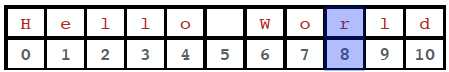
\includegraphics[width=0.6\columnwidth]{string_index}
%		\end{center}
		\begin{itemize}
			\item Can alternatively be negatively indexed $\rightarrow$ last character starts with index of $-1$
		\end{itemize}
%		\begin{center}
%			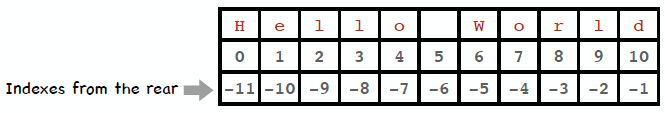
\includegraphics[width=0.6\columnwidth]{string_neg_index}
%		\end{center}
		\begin{itemize}
			\item Slicing of string have the syntax \texttt{[start:stop:step]} with \textcolor{red}{last character being the character before \texttt{stop}}
		\end{itemize}
		\begin{itemize}
			\item Possible to use slicing to reverse a string by doing \texttt{string[::-1]}
		\end{itemize}
		\subsection{Lists}
		\subsubsection{Creation of lists}
		\begin{itemize}
			\item \texttt{furious\_five = ['Tigress', 'Crane', 'Mantis', 'Monkey', 'Viper']}
			\item Can also mix data types in lists e.g. \texttt{numbers = [1, 2.0, 3.0, 4, 5, 6.0]} 
			\item Possible to have empty lists i.e. []
			\item Can create list through type conversion e.g. \texttt{list('abcd')} = ['a', 'b', 'c', 'd'] or \texttt{list(range(5))} = [0, 1, 2, 3, 4]
			\item List comprehension: \mintinline{python}|[expression for item in iterable if conditions]|\newline e.g. \mintinline{python}|[word for word in words if word[0].lower() in 'aeiou']|
			\item Note that \mintinline{python}|list1 = list2| \textcolor{red}{does not actually copy list2 into list1!!}. It just copies a reference to the list $\rightarrow$ any changes made to list2 will affect list1
		\end{itemize}
		\subsubsection{Similarities between Lists and Strings}
		\begin{itemize}
			\item uses the same \texttt{len()} function
			\item uses the same indexing and slicing system
		\end{itemize}
%		\begin{center}
%			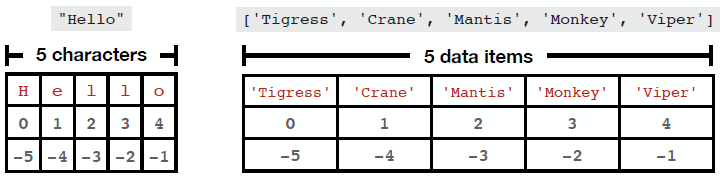
\includegraphics[width=0.6\columnwidth]{string_vs_list}
%		\end{center}
		\subsubsection{Datatypes of list slicing}
		\begin{itemize}
			\item Following the array in the above image, \texttt{type(arr[2])} = str, \texttt{type(arr[2:3])} = list
			and \texttt{type(arr[2:2])} = list (empty list)
		\end{itemize}
		\subsubsection{Difference between String and List}
		\begin{itemize}
			\item Mutability
		\end{itemize}
		\begin{center}
			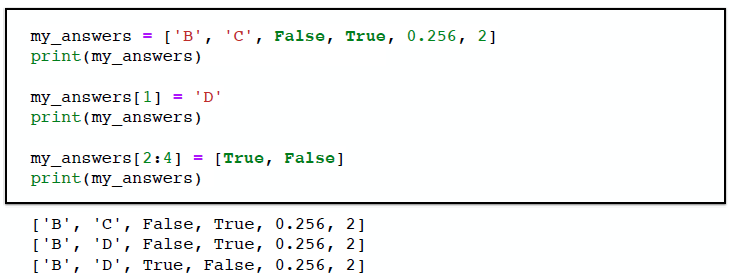
\includegraphics[width=0.6\columnwidth]{list_mutability}
		\end{center}
		\subsubsection{List Methods}
		\begin{itemize}
			\item \texttt{append(item)} - add items to the back of the list
			\item \texttt{extend(list)} - append items from list to another list
			\item \texttt{insert(pos, item)} - insert item at index pos $\rightarrow$ insert new element at \texttt{pos} and shift all elems from \texttt{pos} onwards to the right by 1
%		\begin{center}
%			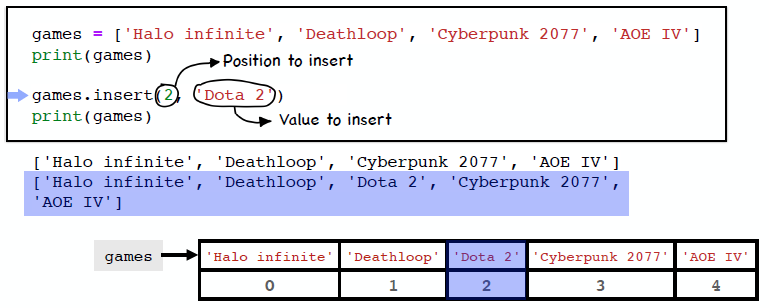
\includegraphics[width=0.7\columnwidth]{list_insert}
%		\end{center}
			\item \texttt{remove(item)} - search and removes the \textcolor{red}{first appearance} of an item in a list, error message is raised if given value is not in list
			\item \texttt{pop(index)} - removes and return the item at index specified, default to last item in list
			\item \texttt{index(item)} - search and returns the index of first appearance of item in list, error raised if item not in list
		\end{itemize}
		\subsubsection{List Comprehension}
		\begin{tabular}{l}
			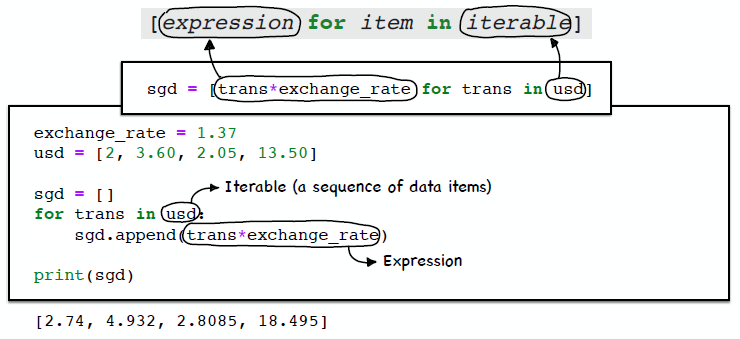
\includegraphics[width=0.45\linewidth]{list_comprehension}
		\end{tabular}
		\begin{tabular}{l}
			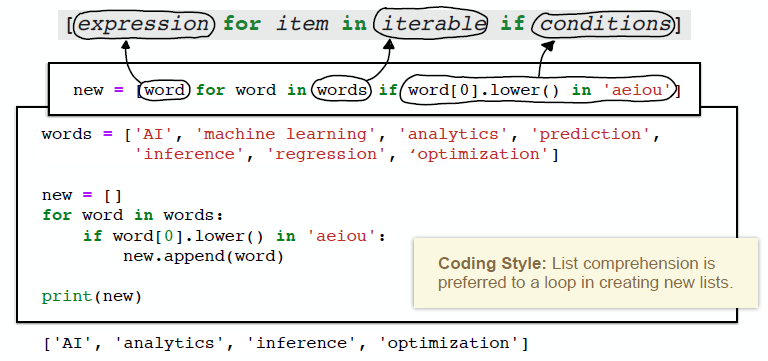
\includegraphics[width=0.45\linewidth]{conditional_list_comprehension}
		\end{tabular} 
		\subsection{Tuples}
		\subsubsection{Tuple Creation}
		\begin{minted}
			{python}
			colors = 'red', 'blue', 'green'
			mixed = ('Jack', 32.5, [1, 2])
			feel_empty = () # empty tuple
			tuple_one = 'here', # tuple
			item_one = ('there') # string
		\end{minted}
		\subsubsection{Features of tuple}
		\begin{itemize}
			\item Immutable
			\item Iterable
			\item Same \mintinline{python}|len()| function, indexing, slicing as strings and lists
			\item Same $+$ and $*$ as strings and lists
			\item \textcolor{red}{No method is defined for tuple}
			\item Tuple unpacking
		\end{itemize}
		\begin{center}
			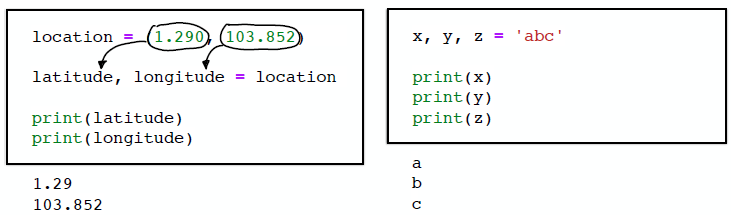
\includegraphics[width=0.7\columnwidth]{tuple_unpacking}
		\end{center}
		\begin{itemize}
			\item \mintinline{python}|zip()| function
			\begin{itemize}
				\item can be applied to other iterable types
				\item can be used to more than 2 data sequences
				\item For sequences with different lengths, the iteration stops when the
				shortest sequence is running out of items
			\end{itemize}
		\end{itemize}
		\begin{center}
			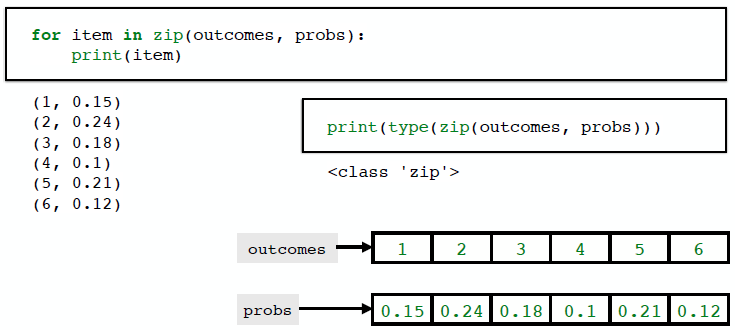
\includegraphics[width=0.7\columnwidth]{zip_tuple}
		\end{center}
		\subsection{Dictionaries}
		\begin{itemize}
			\item Comma-separated $key:value$ pairs enclosed in curly brackets
			\item Keys can be any \textcolor{red}{immutable} types: boolean, integer, float, string, tuple, etc
			\item Values can be any data type
			\item \textcolor{red}{Mutable}
		\end{itemize}
		\subsubsection{Dictionary methods}
		\begin{minipage}{0.6\columnwidth}
			\begin{center}
				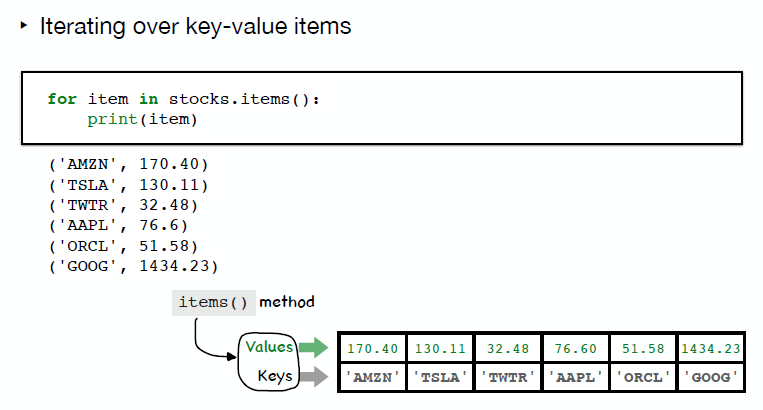
\includegraphics[width=1\columnwidth]{dictionary_methods}
			\end{center}
		\end{minipage}
		\begin{minipage}{0.4\columnwidth}
			\begin{itemize}
				\item \texttt{items()} will get you a (key, value) tuple
				\item \texttt{keys()} will get you all the keys in a list
				\item \texttt{values()} will get you all the values in a list
			\end{itemize}
		\end{minipage}
		\subsection{Summary of data structures}
		\begin{center}
			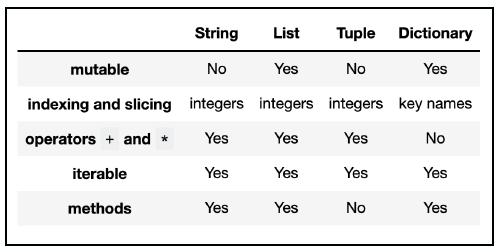
\includegraphics[width=0.7\columnwidth]{ds_summary}
		\end{center}
		\begin{center}
			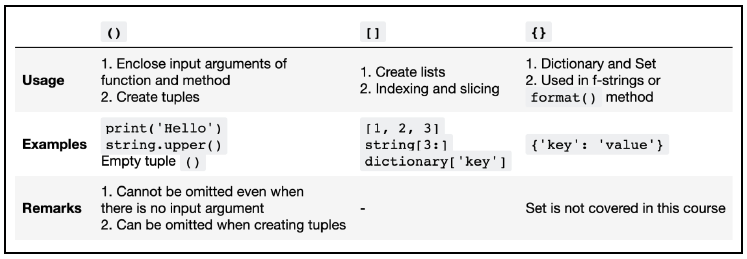
\includegraphics[width=0.7\columnwidth]{parens}
		\end{center}
		\section{Function, Modules, Packages}
		\subsection{Syntax for function names}
		\begin{itemize}
			\item Only 1 word
			\item Only consist of letters, numbers, and underscores
			\item Cannot begin with a number
			\item Avoid contradictions with Python keywords
		\end{itemize}
		\subsection{Syntax of function definition}
		\begin{itemize}
			\item Function terminates when it hits \texttt{return} - will not run any code after \texttt{return} statement
			\item If a function doesn't have a return statement, it \textcolor{red}{implicitly returns \texttt{null}}
		\end{itemize}
		\subsection{Benefits of functions}
		\begin{enumerate}         
			\item Reuse code
			\item Easy to test and debug
			\item Higher readability
		\end{enumerate}
		\subsection{Function arguments and outputs}
		\subsubsection{Positional arguments, keyword arguments and default values}
		\begin{center}
			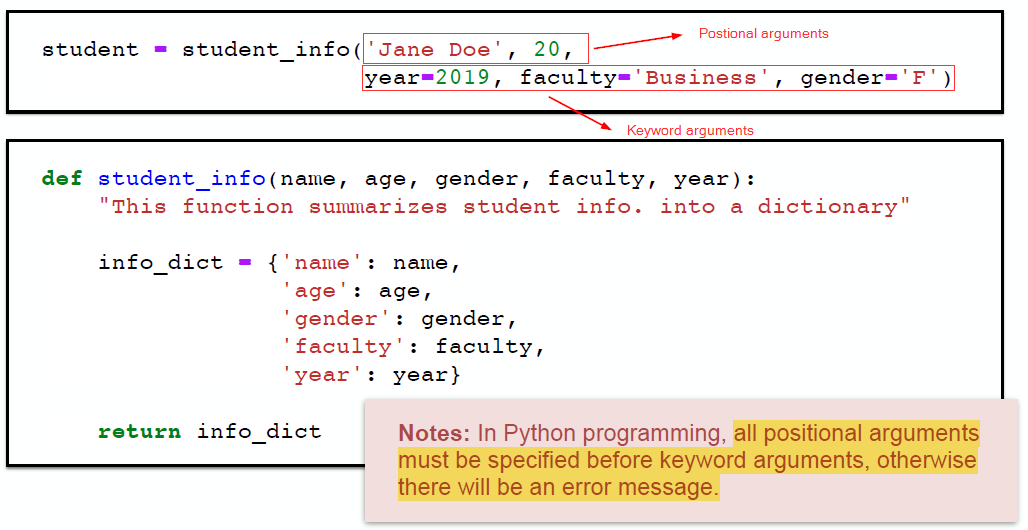
\includegraphics[width=0.7\columnwidth]{func_args}
		\end{center}
		\subsubsection{Multiple Outputs}
		\begin{center}
			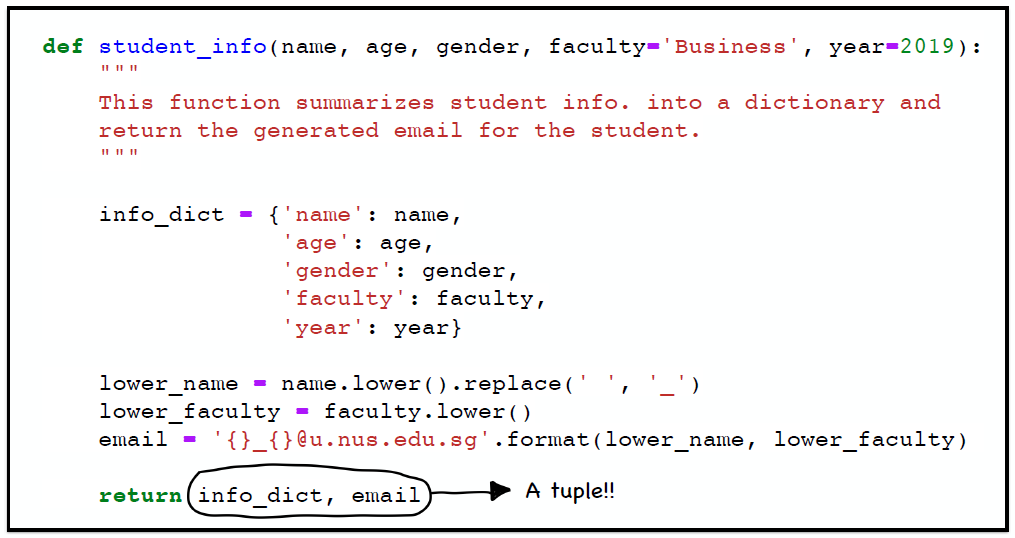
\includegraphics[width=0.7\columnwidth]{mult_out}
		\end{center}
		\subsection{Scopes and namespaces}
		\begin{itemize}
			\item Namespace is a collection of names
			\item The same name may be used to represent different objects in different scopes
			\item Scopes can be defined as follows:
			\begin{itemize}
				\item \textbf{Local}: input arguments and names declared (by assignment statements) in a function and are effective only within the function
				\item \textbf{Global}: names declared outside of function definitions
				\item \textbf{Built-in}: names predefined in Python
			\end{itemize}
		\end{itemize}
		\begin{center}
			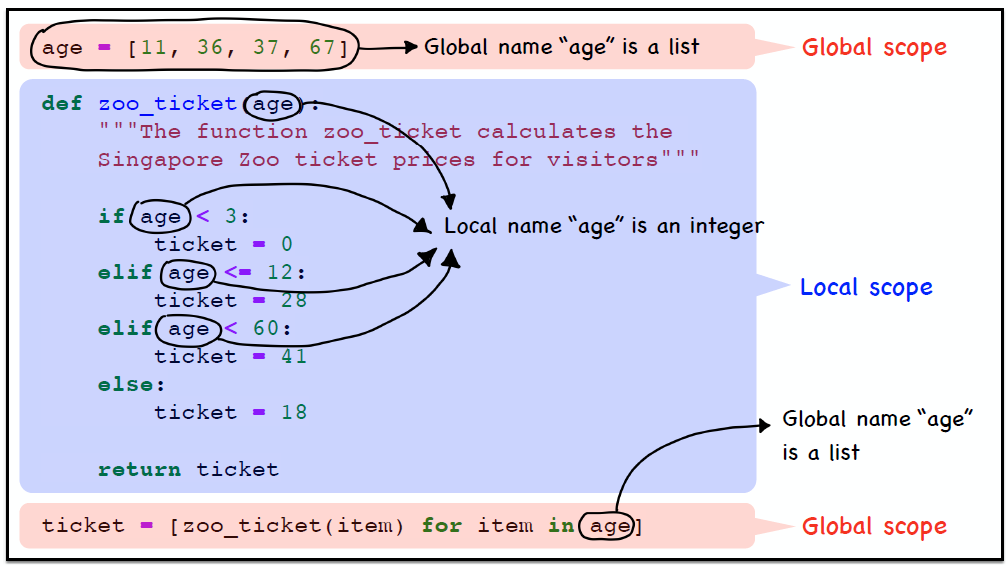
\includegraphics[width=0.7\columnwidth]{scopes}
		\end{center}
		\subsection{Modules}
		A module is a “.py" file that defines functions, classes, variables, or
		simply contains some runnable code.
		\subsubsection{Benefits of Modules}
		\begin{itemize}
			\item Code reuse
			\item System namespace partitioning
			\item Implementing shared services or data
		\end{itemize}
		\subsubsection{Syntax of importing modules}
		\begin{center}
			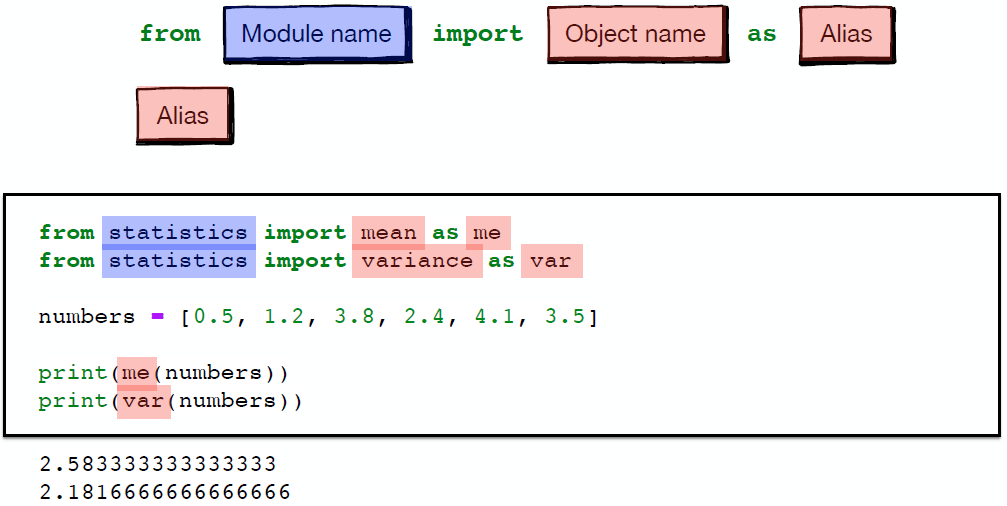
\includegraphics[width=0.7\columnwidth]{modules}
		\end{center}
		\subsection{Packages}
		\begin{itemize}
			\item A collection of modules and supporting files
			\item Use \colorbox{LightGray}{\texttt{.}} operator to indicate the directory hierarchy
		\end{itemize}
		\begin{tabular}{l}
			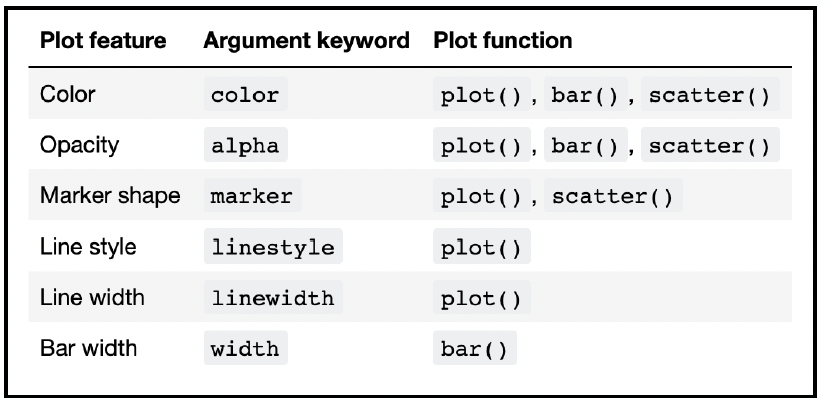
\includegraphics[width=0.47\linewidth]{matplotlib}
		\end{tabular}
		\begin{tabular}{l}
			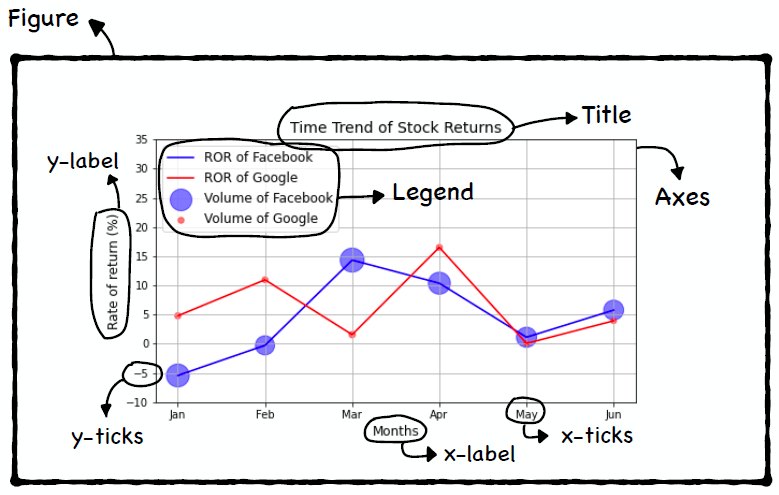
\includegraphics[width=0.45\linewidth]{matplotlib1}
		\end{tabular}
		\section{Lovely Pandas}
		\subsection{Data Representation}
		\begin{itemize}
			\item Variables (fields/attributes) as columns
			\item Observations (cases/records) as rows
		\end{itemize}
		\subsubsection{Types of Variable}
		\begin{itemize}
			\item \textbf{Numerical (Quantitative)} - e.g. things that can be represented with float, int
			\item \textbf{Categorical (qualitative)} - e.g. things that are represented using strings ("M/F"), True/False
			\item Note that True/False can be converted into numerical form by doing \mintinline{python}|int(True/False)| which gives 1/0 respectively
		\end{itemize}
		\subsubsection{Types of Data Situations}
		\begin{itemize}
			\item Could have labeled data
			\item Heterogeneous data - mix of datatypes in the same datasets
			\item Possible missing values - represented by NA in dataset
		\end{itemize}
		\begin{center}
			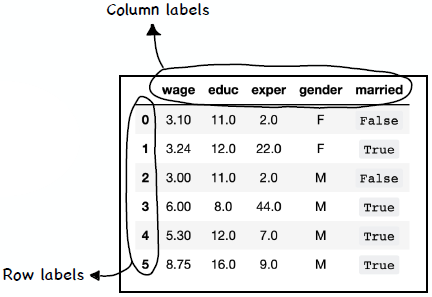
\includegraphics[width=0.5\columnwidth]{pandas_eg}
		\end{center}
		\subsection{\texttt{pandas.Series}}
		\begin{itemize}
			\item 1-dimensional array of indexed data e.g. 1 row or 1 col of dataset
			\item Can be created from a list e.g. \mintinline{python}|wage = pd.Series([3.10, 3.24, 3.00, 6.00, 5.30, 8.75])| or from a tuple e.g. \mintinline{python}|educ = pd.Series((11.0, 12.0, 11.0, 8.0, 12.0, 16.0))|
			\begin{itemize}
				\item Note that the data type of the series will be automatically converted to \texttt{float64}
			\end{itemize}
		\end{itemize}
		\subsubsection{Attributes}
		\begin{center}
			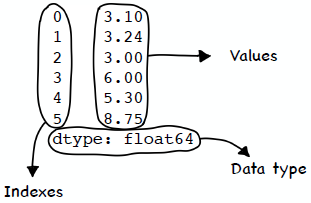
\includegraphics[width=0.5\columnwidth]{pandas_attri}
		\end{center}
		\underline{Index}
		\begin{itemize}
			\item accessed using the \texttt{series.index} attribute
			\item Can specify indexes using an array of values
			\item \texttt{series.index} returns for e.g. \texttt{Index(['Mary', 'Ann', 'John', 'David', 'Frank', 'Ben'], dtype='object')}
		\end{itemize}
		\begin{center}
			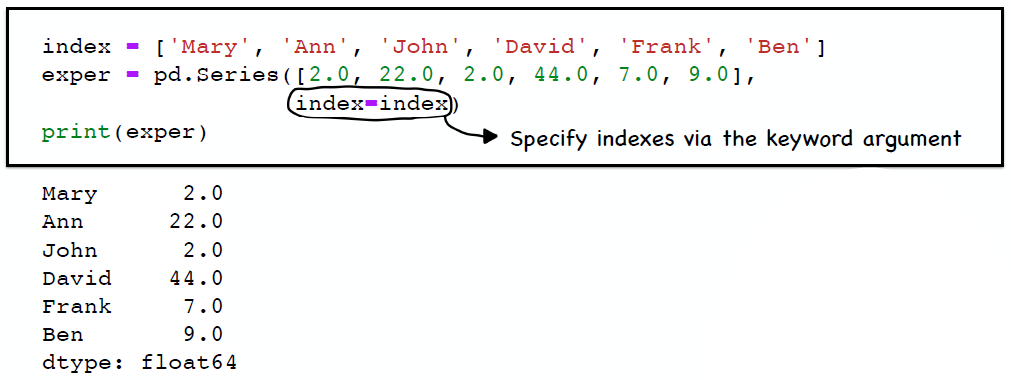
\includegraphics[width=0.5\columnwidth]{series_index}
		\end{center}
		\underline{dtypes}
		\begin{itemize}
			\item \texttt{series.dtype} will return the datatype of the values in the series
			\item In this course: \textcolor{red}{No difference between 64 bit and 32 bit values}
		\end{itemize}
		\begin{center}
			\begin{tabular}{ |c|c| } 
				\hline
				Pandas \texttt{dtype} & Built-in Python types \\ \hline
				\texttt{object} & \texttt{str} or mixed types \\ \hline
				\texttt{int64} & \texttt{int} \\ \hline
				\texttt{float64} & \texttt{float} \\ \hline
				\texttt{bool} & \texttt{bool} \\ 
				\hline
			\end{tabular}
		\end{center}
		\begin{itemize}
			\item can convert the dtype to other types by using the \texttt{series.astype(<type>)} method
		\end{itemize}
		\subsubsection{Series indexing and Slicing}
		\begin{itemize}
			\item indexing and slicing is done by the \texttt{series.iloc[]} and \texttt{series.loc[]} methods
			\item \textcolor{red}{Slicing using \texttt{iloc[]} method does not include the selection index by stop index but slicing using the \texttt{loc[]} method includes the selection indexed by end index}
		\end{itemize}
		\begin{tabular}{l}
			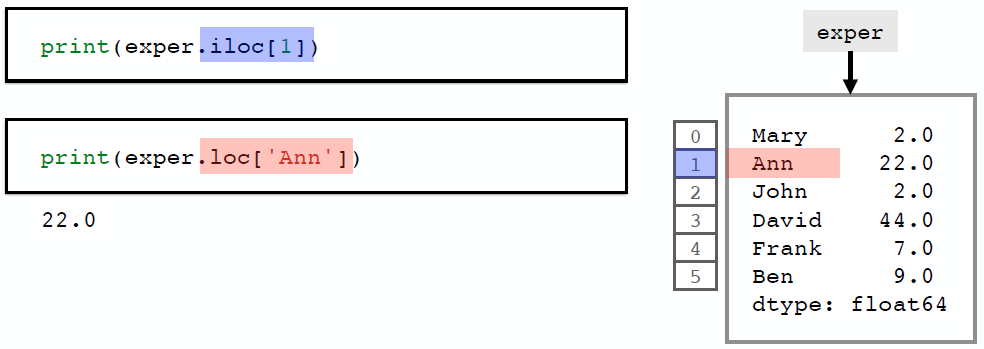
\includegraphics[width=0.45\linewidth]{series_indexing}
		\end{tabular}
		\begin{tabular}{l}
			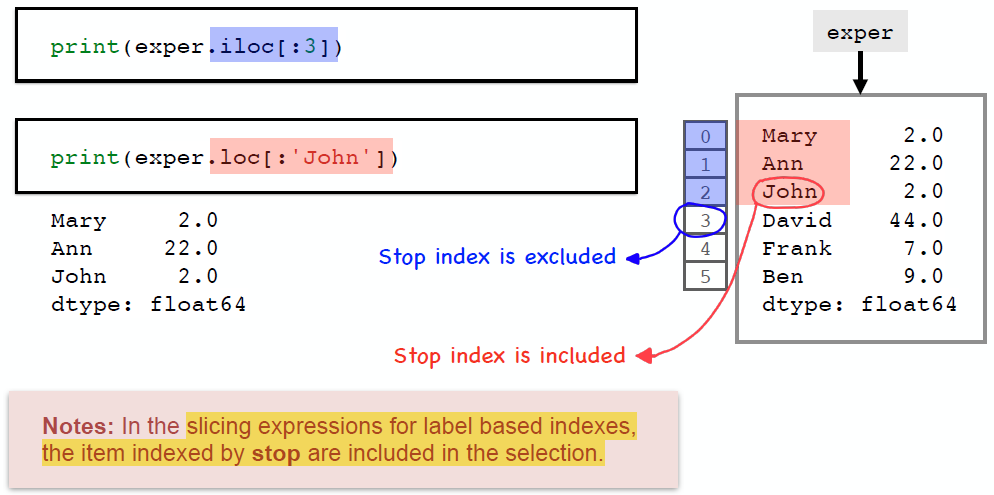
\includegraphics[width=0.45\linewidth]{series_slicing}
		\end{tabular}
		\begin{itemize}
			\item Can also select specific rows/indexes to extract out
		\end{itemize}
		\begin{center}
			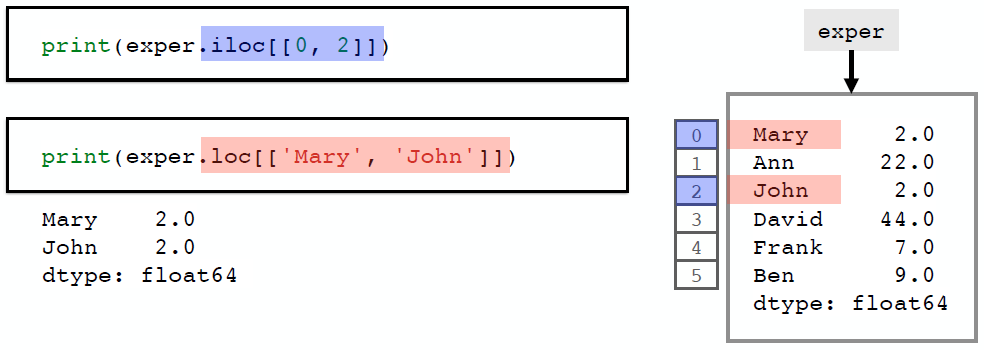
\includegraphics[width=0.5\columnwidth]{series_slicing_spec}
		\end{center}
		\subsection{\texttt{pandas.DataFrame}}
		\begin{itemize}
			\item Dataframe can be created by calling the pd.DataFrame(dict)
		\end{itemize}
		\begin{center}
			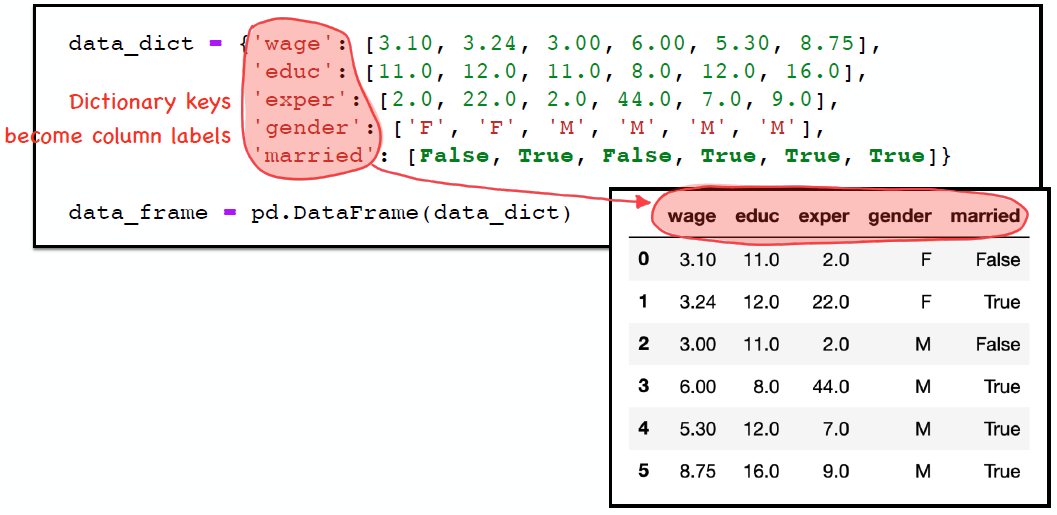
\includegraphics[width=0.6\columnwidth]{dataframe}
		\end{center}
		\begin{itemize}
			\item Has the attributes \texttt{columns} and \texttt{index}
		\end{itemize}
		\begin{center}
			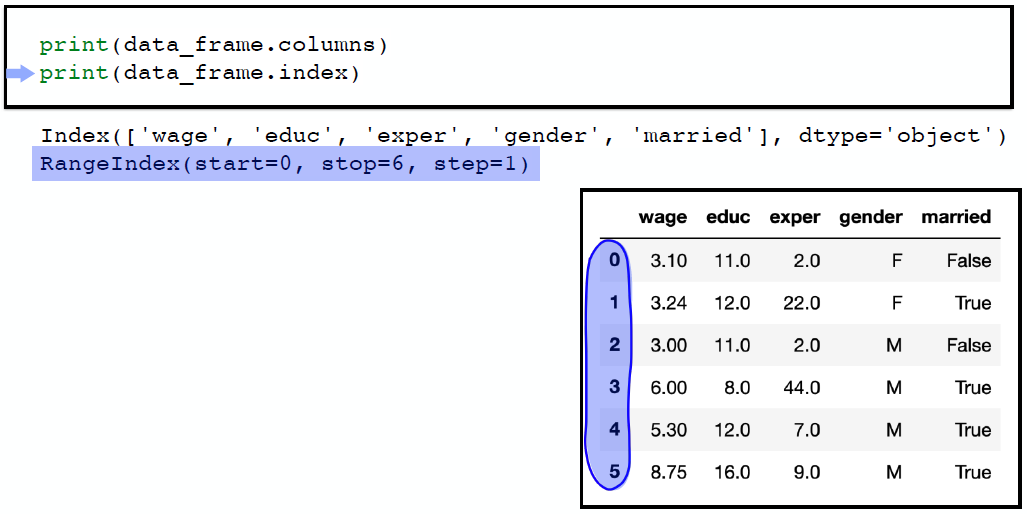
\includegraphics[width=0.5\columnwidth]{dataframe_attri}
		\end{center}
		\begin{itemize}
			\item Can set the index similarly to series
			\item Has the \texttt{dtypes} attribute which returns the \texttt{dtype} of each of the columns
		\end{itemize}
		\subsubsection{Slicing and Indexing of Dataframe}
		\begin{itemize}
			\item Note that the \textbf{default value will be all columns} if columns not specified
		\end{itemize}
		\begin{tabular}{l}
			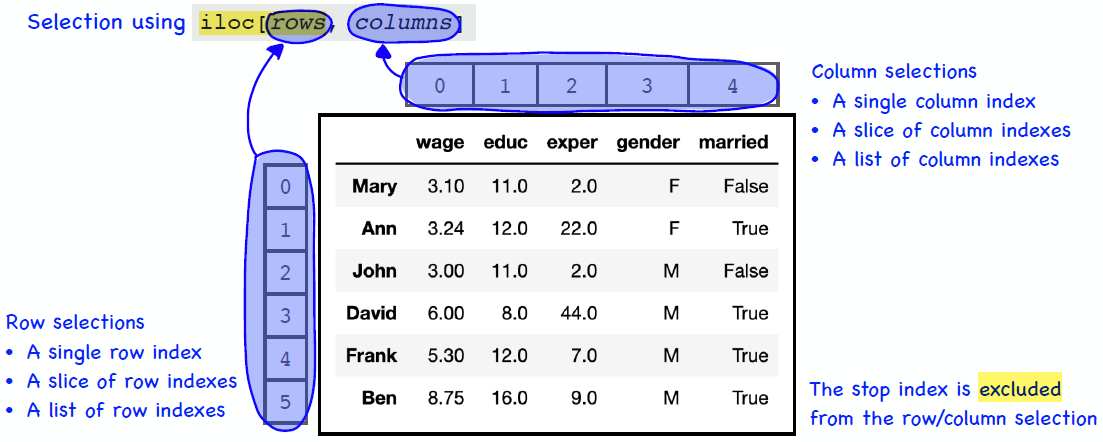
\includegraphics[width=0.49\linewidth]{dataframe_iloc}
		\end{tabular}
		\begin{tabular}{l}
			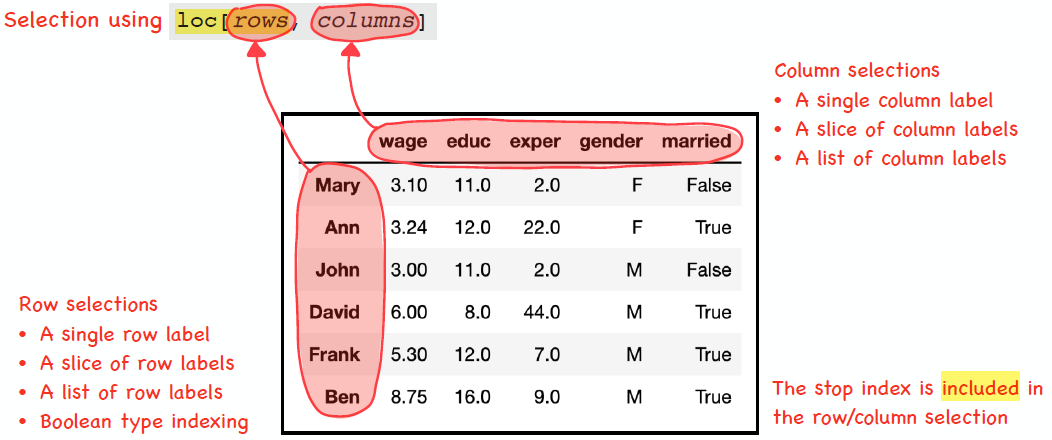
\includegraphics[width=0.49\linewidth]{dataframe_loc}
		\end{tabular}
		\underline{Slicing all rows and specific column / all columns specific rows}
		\begin{tabular}{l}
			\centering
			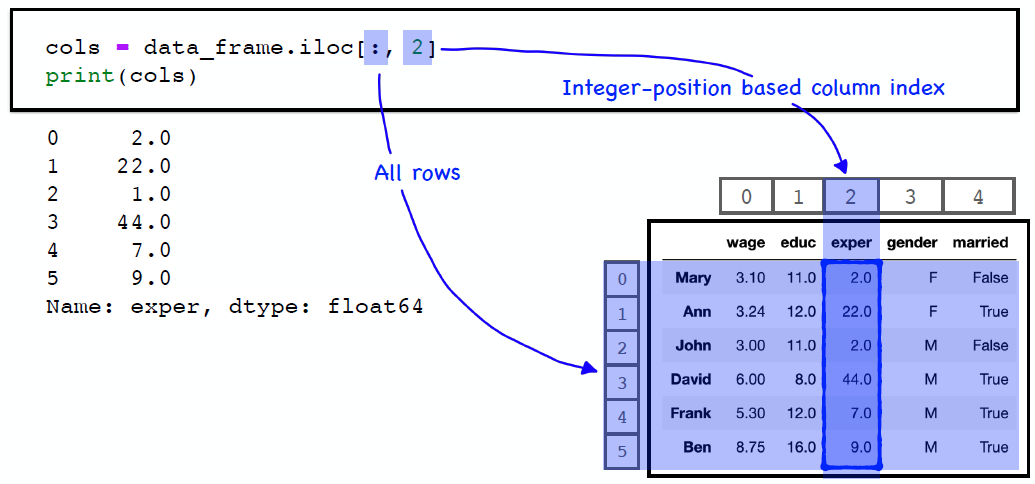
\includegraphics[width=0.48\linewidth]{dataframe_slice}
		\end{tabular}
		\begin{tabular}{l}
			\centering
			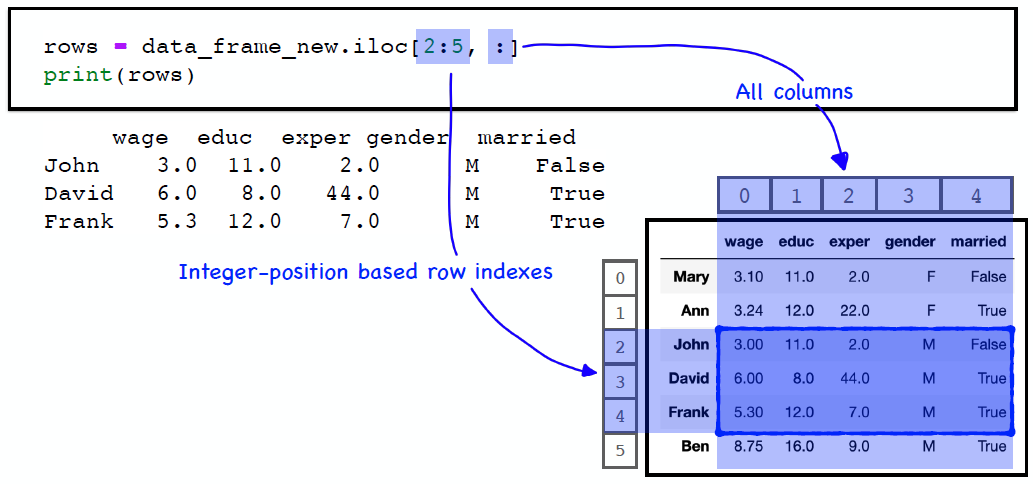
\includegraphics[width=0.47\linewidth]{dataframe_row_slice}
		\end{tabular}
		\begin{center}
			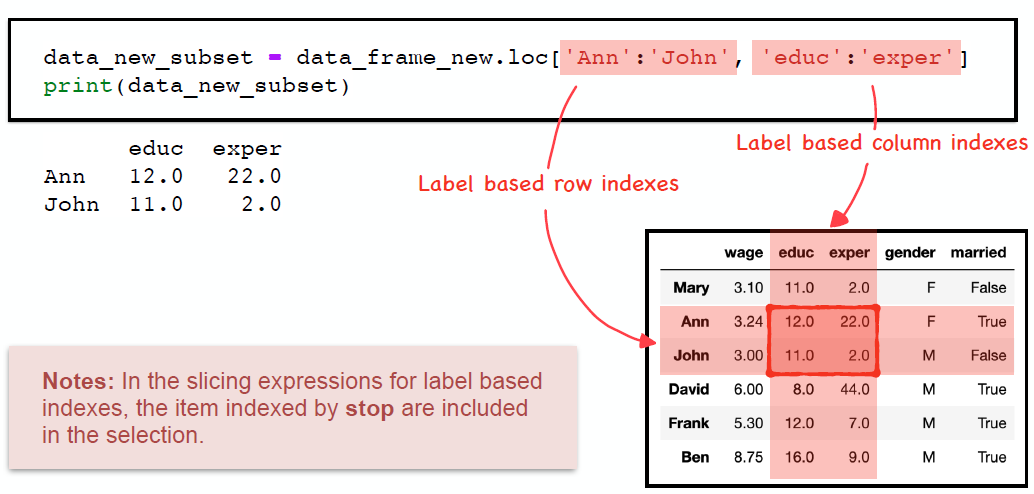
\includegraphics[width=0.6\columnwidth]{dataframe_loc_slice}
		\end{center}
		\underline{Indexing of Column}
		\begin{itemize}
			\item columns of dataframes can be indexed using dataframe['<col\_name>'] 
		\end{itemize}
		\subsubsection{Mutating Dataframes in-place}
		\begin{itemize}
			\item \mintinline{python}|data_frame.loc[2:3, 'educ'] = 9.0 # modifies col 'educ' of rows 2 and 3 to the value 9|
			\item \mintinline{python}|data_frame.iloc[2, 1:3] = 1.0 # changes cols 1 to 2 of row 2 to value of 1.0|
			\item Adding a new column
		\end{itemize}
		\begin{center}
			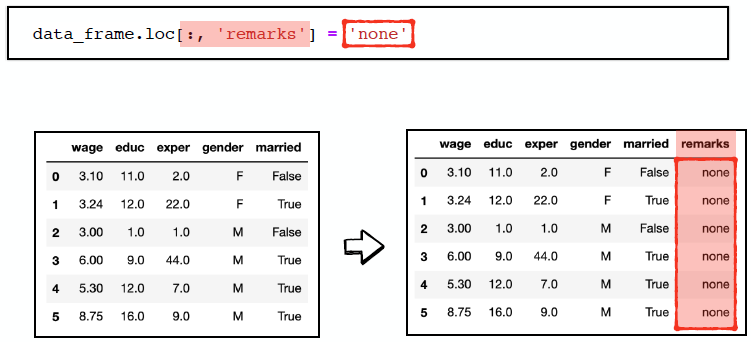
\includegraphics[width=0.5\columnwidth]{dataframe_add_col}
		\end{center}
		\subsubsection{Filtering Data}
		\begin{minipage}{0.55\columnwidth}
			\begin{center}
				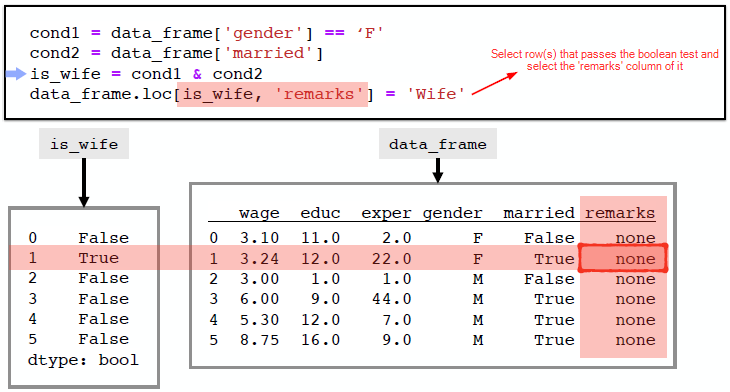
\includegraphics[width=1\columnwidth]{boolean_indexing}
			\end{center}
		\end{minipage}
		\begin{minipage}{0.45\columnwidth}
			\begin{itemize}
				\item Includes other bit-wise manipulation among conditions such as \code{|} for OR operation and $\sim$ for NOT operation
				\item Not operation could alternatively be -ve of the negation e.g. \\
				\mintinline{python}|cond1 = data_frame['gender'] == 'F'|\\
				\mintinline{python}|is_male = -cond1|
			\end{itemize}
		\end{minipage}
		\subsection{Pandas Methods}
		\begin{itemize}
			\item \texttt{pd.read\_csv(csv\_file)} $\rightarrow$ reads a cvs file into a pandas dataframe
			\item \texttt{dataframe.head(6)} $\rightarrow$ shows first 6 records
			\item \texttt{dataframe.drop(columns='gender')} $\rightarrow$ drop the column labeled 'gender'
			\item \textcolor{red}{The following only works if columns are all quantitative values}
			\begin{itemize}
				\item \texttt{dataframe.mean()/median()/mode()} $\rightarrow$ returns the mean/median/mode of each column
				\item \texttt{dataframe.var()/std()} $\rightarrow$ returns the variance/standard deviation of each column 
			\end{itemize}
			\item \texttt{dataframe.min()/max()} $\rightarrow$ returns the min/max values of each column, if comparing \textbf{string} we compare it lexicographically, \textbf{boolean} max will be True and min will be False
			\item \texttt{dataframe[<col>].value\_counts()} $\rightarrow$ returns the count (frequencies) of all unique values
			\item \texttt{dataframe[<col>].value\_counts(normalize=True)} $\rightarrow$ returns the proportions of all unique values, values will add up to 1
			\item \texttt{dataframe.corr()/cov()} $\rightarrow$ returns the correlation/covariance between each column
			\item \texttt{dataframe.describe()} $\rightarrow$ returns count, mean, std, min, 25\%, 50\%, 75\% and max for each col 
			\item \texttt{dataframe[<col>].isnull()/notnull()} $\rightarrow$ returns whether values in col is null/notnull
			\item \texttt{dataframe.dropna()} $\rightarrow$ returns a \textcolor{red}{copy} of the data frame without any rows of missing values. \textcolor{red}{Original dataframe remains unchanged}. If we want to modify original dataframe, use the \texttt{inplace=True} argument
			\item \texttt{dataframe.fillna(<val>)} $\rightarrow$ returns a \textcolor{red}{copy} of the dataframe with all NaN values replaced by val, use \texttt{inplace=True} to modify in place
			\item \texttt{dataframe.set\_index(<col>)} $\rightarrow$ sets col to be the index of dataframe
			\item \texttt{dataframe.reset\_index} $\rightarrow$ typically used to rest the integer index after \texttt{dropna()} or filtering, if \texttt{set\_index()} called previously, previous label turns into a column. \textcolor{red}{If \texttt{reset\_index()} called after \texttt{dropna()} the previous integer indexes also becomes a column}. Use \texttt{drop=True} to drop previous labels
		\end{itemize}
		\subsubsection{Element-wise arithmetic operations}
		\begin{itemize}
			\item Allows us to perform arithmetic operations on each of the elements in the dataframe without loops e.g.\\ \mintinline{python}|gdp_new['1980'] / 1000000 # divide each values in col '1980' by 1000000|
			\item Possible to perform arithmetic operations on 2 cols e.g.\\ \mintinline{python}|gdp_new['1981'] - gdp_new['1980'] # takes every value of col '1981' and subtract from it the corresponding value in col '1980'|
			\item To perform string operations on values:
		\end{itemize}
		\begin{minted}{python}
			project = prop['project']
			project_lower = project.str.lower() # changes all values in col 'project' to lowercase
		\end{minted}
		\begin{itemize}
			\item Possible to use any string operation after the \texttt{.str}
			\item Indexing using the \texttt{.str}: e.g.\\ \mintinline{python}|prop['level_from'] = prop['level'].str[:2].astype(int)|
		\end{itemize}
%		\section{Data Visualization}
%		\subsection{Line Graphs}
%		Line graphs have a continuous data along both the y and x axis with the y-axis showing the value of whatever variable we are measuring and the x-axis used to show when we measured it\\
%		\underline{Use Cases}
%		\begin{itemize}
%			\item Comparing lots of data all at once
%			\item Showing changes and trends over time
%			\item Displaying forecast data and uncertainty
%			\item Highlighting anomalies within and across data series
%		\end{itemize}
%		\underline{Ineffective Cases}
%		\begin{itemize}
%			\item Displaying quantities of things
%			\item Working with \textbf{categorical} data
%			\item Making part-to-whole comparison
%			\item Showing sparse datasets
%		\end{itemize}
%		\subsection{Bar Graphs}
%		\begin{center}
%			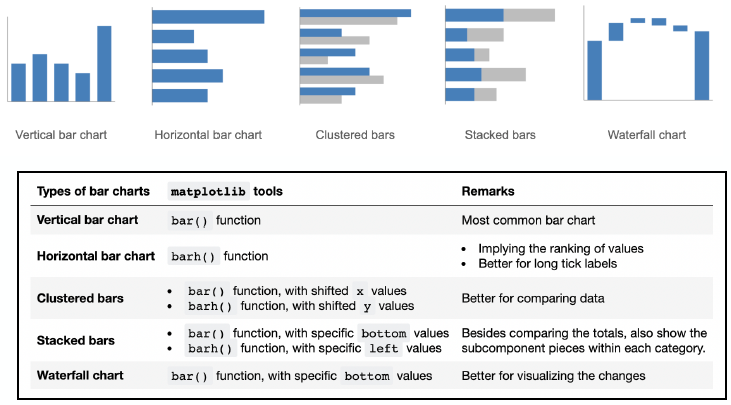
\includegraphics[width=0.7\columnwidth]{bar_graphs}
%		\end{center}
%		\subsection{Scatterplot}
%		A scatterplot is useful for showing the relationship between
%		two things, while a bubble plot is commonly used to visualize relationships between three or more numeric variables
%		\begin{center}
%			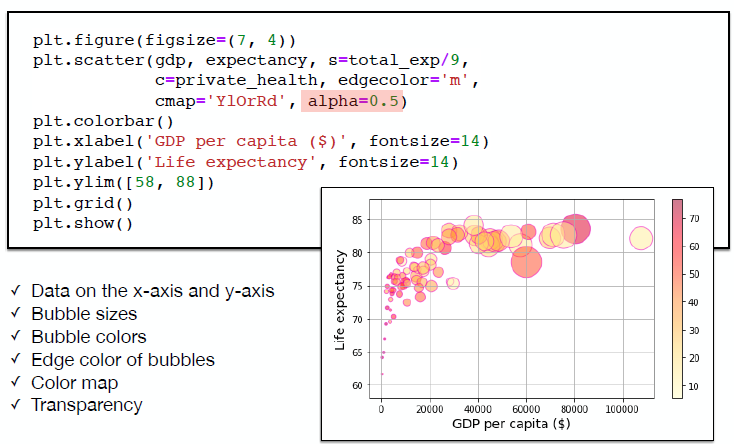
\includegraphics[width=0.7\columnwidth]{bubble_plot}
%		\end{center}
		\section{Numpy}
		\begin{itemize}
			\item Supports the representation of array-like objects like range, list, tuple, series and dataframe
		\end{itemize}
		\begin{center}
			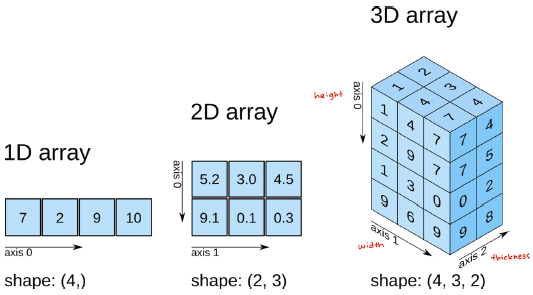
\includegraphics[width=0.5\columnwidth]{N-dim-array}
		\end{center}
		\begin{itemize}
			\item pandas uses numpy internally e.g. \texttt{type(dataframe.values)} is actually of type \texttt{<class 'numpy.ndarray'>}
		\end{itemize}
		\subsection{Attributes of Numpy}
		\begin{itemize}
			\item \texttt{ndim} $\rightarrow$ dimension number of the array
			\item \texttt{shape} $\rightarrow$ shape of array, given as \textbf{tuple}, e.g. 1-dim array will have value (6,), 2-dim array will have value (6, 5). Can be accessed using array.shape[0] which gives row count
			\item \texttt{size} $\rightarrow$ total number of items e.g. 2-dim array with shape of (6, 5) will have value of 30
			\item \texttt{dtype} $\rightarrow$ data type of all data items
		\end{itemize}
		\subsection{Creation of Numpy Arrays}
		\begin{itemize}
			\item Creating a 1d array: \mintinline{python}|array_1d = np.array([61, 52.5, 71, 32.5, 68, 64])|
			\item Creating a 2d array: \mintinline{python}|array_2d = np.array([[18, 26, 17], [25, 15.5, 12], [24, 27, 20], [10, 5.5, 17], [27, 26, 15],	[22, 21, 21]])|
			\item Creating array with all 1s: \mintinline{python}|ones_1d = np.ones(5) # returns array([1., 1., 1., 1., 1.])|
			\item Creating array with all 0s: \mintinline{python}|ones_1d = np.zeros((3, 4)) # returns array([[0., 0., 0., 0.], [0., 0., 0., 0.], [0., 0., 0., 0.]])|
			\item Creating a range of floating point numbers: \mintinline{python}|range_array = np.arange(2, 5, 0.5) # returns array([2. , 2.5, 3. , 3.5, 4. , 4.5])|
			\begin{itemize}
				\item Note that while \texttt{range()} creates a \textbf{range} object, \texttt{arange()} creates a \textbf{ndarray} object
				\item \texttt{range()} can only \textbf{create sequence of integer} while \texttt{arange()} can \textbf{create sequence of any real number}
			\end{itemize}
		\end{itemize}
		\subsection{Indexing and slicing}
		\begin{itemize}
			\item 1d array follows normal slicing and indexing of arrays
			\item 2d array could be sliced using [row, col] e.g. \texttt{array\_2d[3:5, 1:]} will give rows 3,4 and col 1 to the last col, \texttt{array\_2d[[0, 2, 1], 1:]} will give row 0,2,1 and col 1 to the last col
		\end{itemize}
		\subsection{Vectorized Operation}
		\begin{itemize}
			\item Similarly to pandas dataframe, we can run element-wise arithmetic operations on them
			\item Allows for code to be more concise, easier to read and executes faster
			\item Possible to perform arithmetic operations on 2 numpy arrays with same shape too
		\end{itemize}
		\begin{tabular}{l}
			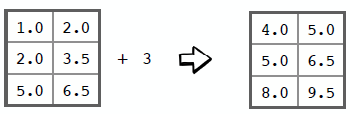
\includegraphics[width=0.37\linewidth]{numpy-op}
		\end{tabular}
		\begin{tabular}{l}
			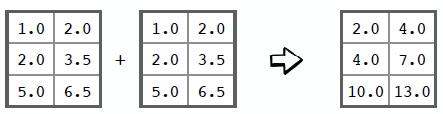
\includegraphics[width=0.45\linewidth]{numpy-array-op}
		\end{tabular}
		\begin{itemize}
			\item Possible to perform arithmetic operation on 2 arrays with different shape by doing \textcolor{red}{broadcasting}
			\begin{itemize}
				\item Note that broadcasting only works with you are duplicating a \textbf{1d array} (either 1 row / col) and does not work with n-dim array (n row / col)
			\end{itemize}
		\end{itemize}
		\begin{center}
			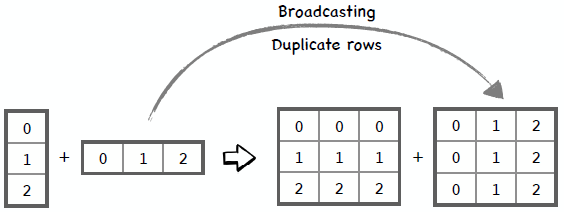
\includegraphics[width=0.4\columnwidth]{broadcasting}
		\end{center}
		\begin{itemize}
			\item When operating on arrays with 2 different shapes, it is also possible to use the \texttt{reshape()} method to change the shape of the array
			\begin{itemize}
				\item for e.g. if you had an array of 10 elem, you could call \texttt{x\_array.reshape(2, 5)} to change the shape of array to a shape of 2 rows, 5 cols
				\item Note that reshaping \textbf{must maintain the size of the original array}, i.e. if original array 10 elems, you cant do \texttt{array.reshape(3,5)}
			\end{itemize}
		\end{itemize}
		\begin{center}
			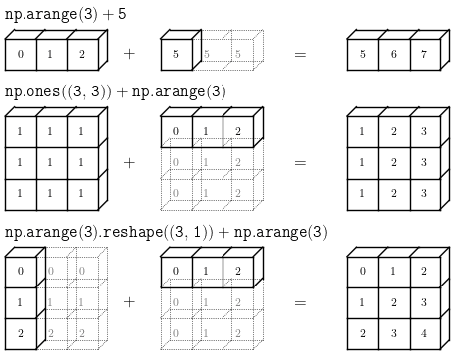
\includegraphics[width=0.4\columnwidth]{reshape}
		\end{center}
		\subsection{Numpy methods}
		\begin{itemize}
			\item \texttt{np.log(<arr or num>)} $\rightarrow$ logs each value in array
			\item \texttt{np.exp(<arr or num>)} $\rightarrow$ gets value of $e^i$ for $i\in $ arr
			\item \texttt{np.square(<arr or num>)} $\rightarrow$ get value of $i^2$ for each $i\in$ arr
			\item \texttt{np.power(<power>, <arr or num>)} $\rightarrow$ gets the value of $i^{power}$ for each $i \in$ arr
			\item \texttt{np.cos()/sin()}
			\item Supports all of \texttt{sum(), max()/min(), mean(), var()/std()}, \texttt{var()/std()} calculates the \textbf{population var or std }by default
			\item Can specify the axis to aggregate by passing as args, \texttt{axis=0} is col while \texttt{axis=1} is row
		\end{itemize}
		\section{Review of Probability}
		\subsection{General Probability Rules}
		\begin{itemize}
			\item Rules of complement: $P(A) = 1 - P(A^c)$, where $A^c$ is the complement of $A$
			\item General addition rule: $P(A_1 \text{ or } A_2) = P(A_1) + P(A_2) - P(A_1 \text{ and } A_2)$, if $A_1$ and $A_2$ are \textcolor{red}{mutually exclusive} then $P(A_1 \text{ or } A_2) = P(A_1) + P(A_2)$
			\item Conditional Probability: $P(A|B)=\frac{P(A \text{ and } B)}{P(B)} \rightarrow P(A \text{ and } B) = P(A|B)P(B)$, if $A$ and $B$ are \textcolor{red}{independent } then $P(A \text{ and } B)=P(A)P(B)$
		\end{itemize}
		\subsection{Discrete Random Variables}
		\begin{itemize}
			\item Refers to variables with possible outcomes being finite are countable
			\item e.g. Preference of coke or pepsi, result of dice roll, number out of $x$ people who prefer Coke over Pepsi (\textbf{binomial}), The number of patients arriving in an emergency room within a fixed time interval (\textbf{poisson})
		\end{itemize}
		\subsubsection{Probability Mass Function (PMF)}
		Point Probability. Given as $P(X=x_j)=p_j$ for each $j=1,2,\cdots,k$ where $p$ must satisfy
		\begin{equation*}
			\begin{cases}
				0\leq p_j \leq 1 & \text{for each } j = 1,2,\cdots,k\\
				\sum_{j=1}^{k}p_j=1
			\end{cases}
		\end{equation*}
		\subsubsection{Binom example}
		\begin{minted}{python}
			from scipy.stats import binom
			x = 8 # test variable, could be an array
			n = 10 # size of sample
			p = 0.65 # probability of event happening
			
			pmf = binom.pmf(x, n, p)
		\end{minted}
		\subsection{Cumulative Distribution Function (CDF)}
		The CDF of a random variable $X$ is defined as $F(x) = P(X \leq x)$, $F(x) \leq 1$. Can be understood as the probability of an event happening $\leq X$ times. In discrete variables, graph would typically look like a staircase
		\begin{itemize}
			\item In questions that asks "what is the probability that at least $x$ ...", we could either do \texttt{1-<distribution>.cdf(x-1, p)} OR \texttt{<distribution>.cdf(x, 1-p)}
		\end{itemize}
%		\subsubsection{Binom example}
%		\begin{center}
%			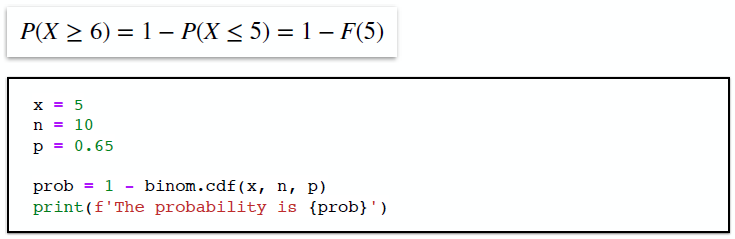
\includegraphics[width=0.6\columnwidth]{cdf}
%		\end{center}
		\subsection{Continuous Random Variables}
		\begin{itemize}
			\item Refers to variables where it could take all values in an interval of numbers
		\end{itemize}
		\begin{center}
			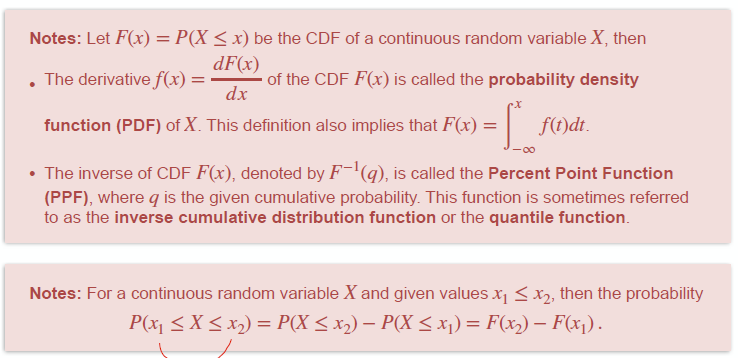
\includegraphics[width=0.7\columnwidth]{crv}
		\end{center}
		\begin{itemize}
			\item Note that for Continuous Random Variable, there is no concept of $P(x_1=X)$ and $P(x_1=X)$ is always = 0
		\end{itemize}
		\subsubsection{Normal example}
		\begin{minted}{python}
			from scipy.stats import norm
			x = -30 
			mean = 20.6
			std = 30.85 
			
			pmf = norm.cdf(x, mean, std)
		\end{minted}
		\subsubsection{Percent Point Function}
		\begin{itemize}
			\item Could be understood as asking: What is the actual value that will cause $x_1$ to occur with a probability $\geq X$
		\end{itemize}
		\subsection{Expected Value and Variance}
		\begin{center}
			\begin{tabular}{ |c|c|c| } 
				\hline
				& Discrete & Continuous \\ \hline
				$\mathbb{E}$(X) & $\sum_{i=1}^{k}x_ip_i$ & $\int_{x\in \mathscr{X}}xf(x)dx$ \\ \hline
				\text{Var}(X) & $\sum_{i=1}^{k}(x_i-\mathbb{E}(X))^2p_i$ & $\int_{x\in \mathscr{X}}(x-\mathbb{E}(X))^2f(x)dx$\\ 
				\hline
			\end{tabular}
		\end{center}
		\begin{center}
			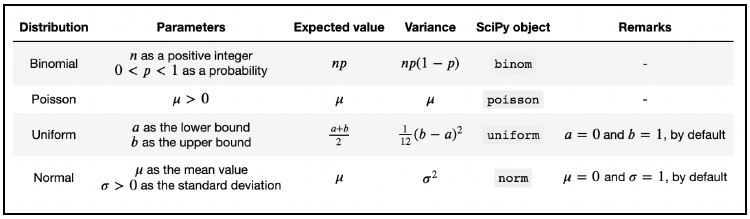
\includegraphics[width=0.8\columnwidth]{expected}
		\end{center}
		\subsubsection{Properties of Expected Value and Variances}
		\begin{itemize}
			\item $\mathbb{E}(c)=c$
			\item $\mathbb{E}(aX+c)=a\mathbb{E}(X)+c$
			\item $\mathbb{E}\left(\sum_{i=i}^{n}a_iX_i\right)=\sum_{i=1}^{n}a_i\mathbb{E}(X_i)$
			\item Var($c$) = 0
			\item Var($aX+c$)=$a^2$Var($X$), Note that $Cov(X, X) = Var(X)$
			\item Var($aX+bY+c$) = $a^2\text{Var}(X)+b^2\text{Var}(Y)+2ab\text{Cov}(X,Y)$, if all random variables are \textbf{pairwise independent}: $\text{Var}\left(\sum^{n}_{i=1}a_iX_i\right)=\sum_{i=1}^{n}a_i^2\text{Var}(X_i)$
		\end{itemize}
		\subsubsection{Log returns}
		\begin{center}
			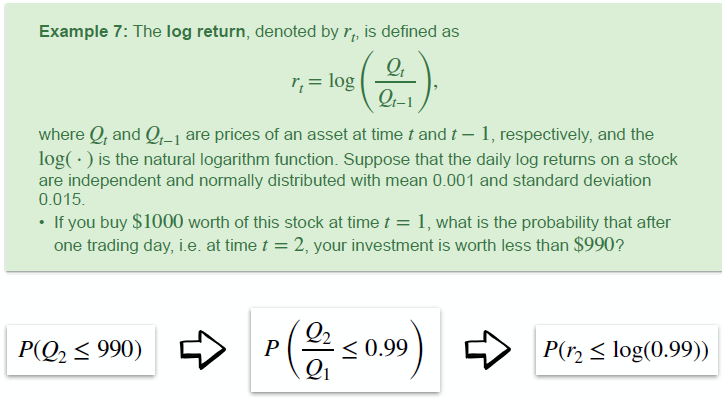
\includegraphics[width=0.6\columnwidth]{log-returns}
		\end{center}
		\begin{itemize}
			\item One nice property of log returns is that regardless of what $t$ is, the returns will always be $\log\left(\frac{Q_t}{Q_1}\right)$
		\end{itemize}
		\begin{center}
			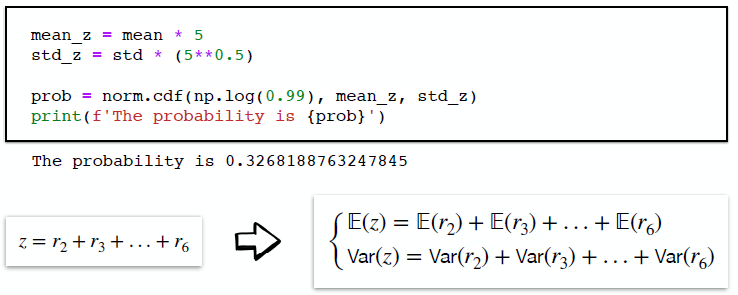
\includegraphics[width=0.55\columnwidth]{log-returns-t6-2}
		\end{center}
		\section{Random Sampling}
		\begin{itemize}
			\item \textbf{Population}: the collection of all individuals or items under consideration in a statistical study $\rightarrow$ impractical to study whole population due to \textbf{time and cost constraints}
			\item \textbf{Sample}: part of the population from which information is obtained
		\end{itemize}
		\subsection{Population parameters and Sample Statistics}
		\begin{center}
			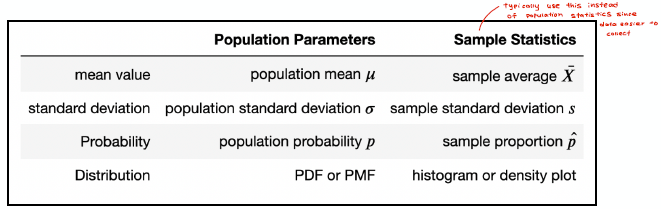
\includegraphics[width=0.7\columnwidth]{pop-vs-sam}
		\end{center}
		\begin{center}
			\begin{tabular}{|l|l|l|}
				\hline
				& Population & Sample\\ \hline
				Mean & $\mu=\begin{cases}
					\displaystyle\sum_{i=1}^{k}x_ip_i\\
					\int_{x\in \mathscr{X}}xf(x)dx
				\end{cases}$ & $\bar{X}=\frac{1}{n}\displaystyle\sum_{i=1}^{n}X_i$\\ \hline
				Variance & $\sigma^2=\begin{cases}
					\displaystyle\sum_{i=1}^{k}(x_i-\mathbb{E}(X))^2p_i\\
					\int_{x\in \mathscr{X}}(x-\mathbb{E}(X))^2f(x)dx
				\end{cases}$ & $s^2=\frac{1}{n-1}\displaystyle\sum_{i=1}^{n}(X_i-\bar{X})^2$ \\ \hline
			\end{tabular}
		\end{center}
		\subsection{Central Limit Theorem}
		\begin{itemize}
			\item For a relatively large sample size, the random variable $\bar{X}=\frac{1}{n}\displaystyle\sum_{i=1}^{n}X_i$ is \textcolor{red}{approximately normal distributed}, regardless of distribution of population. Approximation becomes better with increased sample size.
		\end{itemize}
		\section{Confidence Interval and Hypothesis Testing}
		\subsection{Review of Sampling Distribution}
		\begin{itemize}
			\item $\mathbb{E}(\bar{X})=\mathbb{E}\left(\frac{1}{n}\displaystyle\sum_{i=1}^{n}X_i\right)=\frac{1}{n}\displaystyle\sum_{i=1}^{n}\mathbb{E}(X_i)=\frac{1}{n}\displaystyle\sum_{i=1}^{n}\mu=\mu$
			\item Var$(\bar{X})=$Var$\left(\frac{1}{n}\displaystyle\sum_{i=1}^{n}X_i\right)=\frac{1}{n^2}\displaystyle\sum_{i=1}^{n}$Var$(X_i)=\frac{1}{n^2}n\sigma^2=\frac{\sigma^2}{n}$
		\end{itemize}
		\subsection{Confidence Interval}
		\begin{itemize}
			\item \textbf{General idea}: There are many \textit{point estimates around the population mean} and each of the point estimates can \textit{exist in a range of plausible value} (depending on sample or population std)
			\item \textbf{Confidence Interval} is given by the equation: \texttt{estimate $\pm$ margin of error}
			\begin{itemize}
				\item Note that if population std is known, \textbf{margin of error will be the same for each point estimate}
			\end{itemize}
		\end{itemize}
		\subsubsection{Confidence Interval when $\sigma$ is known}
		\begin{itemize}
			\item $\bar{X}$ is approximately normally distributed (by CLT)
			\item Mean value of $\bar{X}$ is the population mean $\mu$
			\item Std of $\bar{X}$ is $\sigma/\sqrt{n}$
			\item $z-$value: $\dfrac{\bar{X}-\mu}{\sigma/\sqrt{n}}\sim N(0,1)$
			\item \textbf{Interval}: $\bar{X}\pm\frac{\sigma}{\sqrt{n}}\cdot z_{\alpha/2}\rightarrow$ \textcolor{red}{Alt Upper bound:} \texttt{x\_bar-norm.ppf(alpha/2)*se}
			\item $\frac{\sigma}{\sqrt{n}}$ is known, only need to calculate $z_{\alpha/2}$ $\rightarrow F^{-1}(1-\alpha/2)$ (PPF of $\alpha/2$)
			\item Code: \mintinline{python}|z_alpha2 = scipy.stats.norm.ppf(1-alpha/2)|
		\end{itemize}
		\begin{center}
			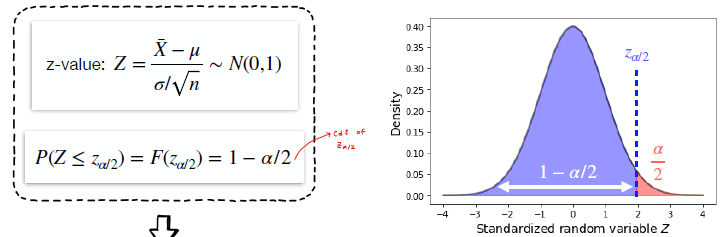
\includegraphics[width=0.6\columnwidth]{conf-interval-known}
		\end{center}
		\subsubsection{Confidence Interval when $\sigma$ is unknown}
		\begin{itemize}
			\item $t-$value: $T=\dfrac{\bar{X}-\mu}{s/\sqrt{n}}\sim t-$distribution $\rightarrow$ tends to $Z-$distribution as $n$ increases (Degree of Freedom ($n$-1) increases)
			\item \textbf{Interval}: $\bar{X}\pm\dfrac{s}{\sqrt{n}}\cdot t_{\alpha/2}$
			\item Code: \mintinline{python}|t_alpha2 = scipy.stats.t.ppf(1-alpha/2, n-1)|
		\end{itemize}
		\subsection{Confidence Interval for Proportions}
		\begin{itemize}
			\item Population proportion: $p$, Sample proportion: $\hat{p}=\frac{m}{n}$
			\item $\mathbb{E}(\hat{p})=\mathbb{E}\left(\frac{m}{n}\right)=\frac{\mathbb{E}(m)}{n}=\frac{np}{n}=p$
			\item Var($\hat{p})=$Var$\left(\frac{m}{n}\right)=\frac{\text{Var}(m)}{n^2}=\frac{np(1-p)}{n^2}=\frac{p(1-p)}{n}\rightarrow$ Var$(\hat{p})$ decreases as $n$ increases
			\item Shape of sampling distribution approaches normal as $n$ increases
			\item \textbf{Interval}: $\hat{p}\pm\sqrt{\frac{\hat{p}(1-\hat{p})}{n}}\cdot z_{a/2}$$\rightarrow$ max margin of error is when $\hat{p}(1-\hat{p})=0.5$
		\end{itemize}
		\subsection{Hypothesis Testing}
		\begin{itemize}
			\item 3 types of tests: 2-tailed test - $H_a:\mu\neq\mu_0$, Left-tailed - $H_a:\mu<\mu_0$, Right-tailed - $H_a:\mu>\mu_0$
			\item General steps: 
			\begin{minted}{python}
				n = <no. of samples>
				alpha = <significance level>
				mu0 = <null hypothesis>
				t_value = (x_bar - mu0) / (sample_std / n ** 0.5)
			\end{minted}
			\item If right-tailed test: \mintinline{python}|p_value = 1 - t.cdf(t_value, n-1)|
			\item If left-tailed test: \mintinline{python}|p_value = t.cdf(-t_value, n-1)|
			\item If 2-tailed test: \mintinline{python}|p_value = 2 * (1 - t.cdf(t_value, n-1))| OR \mintinline{python}|p_value = 2 * (t.cdf(-t_value, n-1))|
			\item If p\_value > alpha, \textbf{reject alternative hypothesis} in favor of null hypothesis
			\item If p\_value < alpha, \textbf{reject null hypothesis} in favor of alternative hypothesis  
		\end{itemize}
		
%		\begin{center}
%			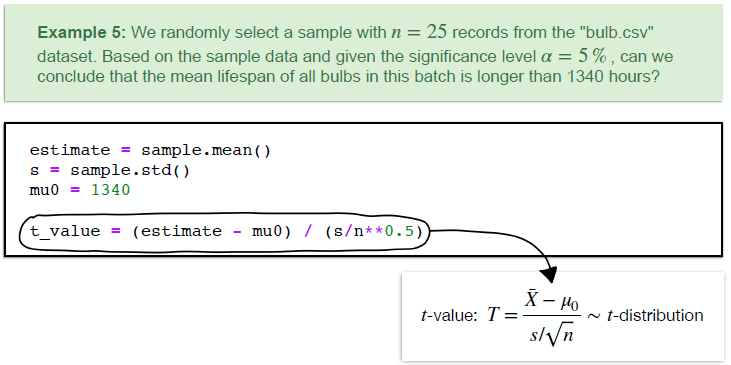
\includegraphics[width=0.6\columnwidth]{hypo-test1}
%		\end{center}
%		\begin{center}
%			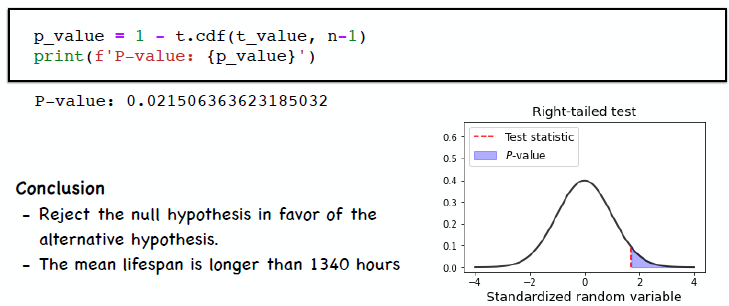
\includegraphics[width=0.6\columnwidth]{hypo-test2}
%		\end{center}
	\end{multicols*} 
\end{document}
